% Draft chapter: heat and kinetics of hydrogen exsolution. Numbers from heat_numbers.tex.

\section{Heat of Hydrogen Exsolution}\label{sec:heat}

Mixing hydrogen into silicate melt absorbs heat: the excess enthalpy of the source
simulations is positive at every composition \cite{gilmore2026data}. Separation therefore
releases heat. We obtain this heat from the same free energy that sets the binodal, by
automatic differentiation in \Atm{} (Appendix~\ref{app:thermo}). The relevant quantity for a
planet is the partial molar enthalpy of H$_2$ in the melt, $\bar h_{\rm H_2}$: the heat
released when a small amount of hydrogen leaves the melt and ends as pure H$_2$.

For the published fit, $\bar h_{\rm H_2}$ is \hbarPubLo{}--\hbarPubHi{}\,MJ per kg of hydrogen
between 1 and 3\,wt\% and 2 and 5\,GPa. The class-M1 refit posteriors that include the
enthalpy data give \hbarMOneLo{}--\hbarMOneHi{}\,MJ\,kg$^{-1}$ (95\% intervals over the same
grid), with medians of \hbarMOneTableOne{} and \hbarMOneTableThree{}\,MJ\,kg$^{-1}$ at 1 and
3\,wt\% and 2\,GPa. In refit M1 ($B/A = \BAMOneTable{}$, so $B < 2A$) the heat is largest for
dilute hydrogen, where each H$_2$ molecule is surrounded by silicate. The published fit
($B/A = 5.65$) instead peaks at $x = 0.26$ ($w = \pubThreshold{}$\,wt\%), where $W''$ changes
sign, and falls to 35\,MJ\,kg$^{-1}$ at infinite dilution and 2\,GPa
(Appendix~\ref{app:energy}). The 1\,wt\% values ($x = 0.20$) lie below the most hydrogen-poor
simulation ($x = 0.24$, 1.2\,wt\%), so they are extrapolations.

The source data favour the refits here. At the most hydrogen-poor simulated mixture
($x = 0.24$, 5.08\,GPa, 4000\,K), the simulated excess enthalpy is
$\edHexData\pm\edHexSig$\,kJ\,mol$^{-1}$ (1$\sigma$, after the endmember pressure correction;
Table~\ref{tab:homogeneous}). The published fit gives \edHexPub{}\,kJ\,mol$^{-1}$,
\edHexPull{} standard deviations too low, and refit M1 gives \edHexMOne{}\,kJ\,mol$^{-1}$. At
$x = 0.83$ the published fit is too high instead (\edHexRichPub{} against
$\edHexRichData\pm\edHexRichSig$\,kJ\,mol$^{-1}$; M1: \edHexRichMOne{}), so its fault is the
asymmetry of the excess. The refit to phase compositions alone, without enthalpy data, predicts
\edHexPhaseComp{}\,kJ\,mol$^{-1}$ at $x = 0.24$ and
\hbarPhaseCompLo{}--\hbarPhaseCompHi{}\,MJ\,kg$^{-1}$; the enthalpy data rule it out.

Per kilogram of hydrogen, this heat is \latentRatioLo{}--\latentRatioHi{} times the latent heat
of melting per kilogram of silicate (0.73\,MJ\,kg$^{-1}$; \cite{tejada2026}). Hydrogen makes up
only 1--3\% of the mass, however, so per kilogram of interior the two heats are comparable.
Over the first 300\,K below the binodal, a 3\,wt\% interior at 2\,GPa (refit M1,
Section~\ref{sec:interior}) releases \intHeatThree{} (\intHeatThreeLo{}--\intHeatThreeHi{})\,MJ
per kg of interior, \latentInteriorThree{} times the latent heat. At 1\,wt\% it releases
\intHeatOne{} (\intHeatOneLo{}--\intHeatOneHi{})\,MJ\,kg$^{-1}$, \latentInteriorOne{} times the
latent heat.

The data constrain the heat only at 4000\,K. Consider an excess heat capacity
$c_{\rm ex} = \pm50\,x(1-x)$\,J\,mol$^{-1}$\,K$^{-1}$ per oxide-basis mole, at most $\pm12.5$ at
$x = 0.5$, with the excess enthalpy held at its simulated value at 4000\,K. At 3000\,K it
changes $\bar h_{\rm H_2}$ by $\mp50\,(1-x)^2$\,kJ\,mol$^{-1}$, lowering it for positive
$c_{\rm ex}$. That is \cexShiftLo{}--\cexShiftHi{}\% of the published and M1 median values
over the same grid, and the shift is largest for dilute hydrogen.

\section{How Far Below the Binodal Separation Starts}\label{sec:kinetics}

The delayed-exsolution window of Section~\ref{sec:window} assumes that a cooling parcel stays
homogeneous until the spinodal. A metastable parcel can instead nucleate the hydrogen-rich
phase. We compute the critical nucleus in square-gradient theory \cite{cahn1958,cahn1959},
using the same free energy, a gradient coefficient $\kappa$ and a constant molar volume. The
barrier scales exactly as $\kappa^{3/2}$, tends to classical theory near the binodal and
vanishes as the 3/2 power at the spinodal (Appendix~\ref{app:thermo}). Nucleation becomes
effective once the barrier falls to $W^*/k_{\rm B}T = \ln(J_0 V t)$ \cite{kashchiev2000}. We
take 69--123. The lower value uses $J_0 = 10^{30}$\,m$^{-3}$\,s$^{-1}$, $V = 1$\,m$^3$ and
$t = 1$\,s. The upper value uses $J_0 = 10^{40}$\,m$^{-3}$\,s$^{-1}$, $V = 1$\,m$^3$ and
$t = 1$\,Myr. A volume of $10^{20}$\,m$^3$ over 1\,Gyr would raise the criterion to 153--176,
which shortens the delays further. The molar volume is 18.2\,cm$^3$ per mole of mixing units,
varied by $\pm30\%$. It is the cell volume of the two-phase run at 2.05\,GPa and 3000\,K in ED
Table~1: 258 atoms of 13.52\,\AA$^3$ over 115.5 mixing units.

The gradient coefficient follows from a simulated two-phase profile. Figure~1c of
\cite{gilmore2026} shows the time-averaged number densities of H, O and Si across the interface
at 10\,GPa and 2500\,K, below the published $T_C$ of \pubTcTen{}\,K there. We fitted their
equation~4 to each species and took the 10--90\% width, $2\,{\rm artanh}(0.8)\,\delta$, which is
0.28--0.33\,nm. If all species share $\delta$ and the centre, the composition $x$ has the same
width, so we use this range for $x$. Each model's free energy at that state converts the width
to $\kappa$ (Appendix~\ref{app:nucleation}). We then hold $\kappa$ fixed at the parcel's
pressure and temperature. Capillary waves and drift of the slab can only broaden a
time-averaged profile, so any broadening makes $\kappa$ and the delays below too large.

With this width, a 3\,wt\% parcel at 2\,GPa nucleates \dlyFigOneCPubLo{}--%
\dlyFigOneCPubHi{}\,K below the binodal for the published fit, and \dlyFigOneCMOneLo{}--%
\dlyFigOneCMOneHi{}\,K below it across the M1 posterior (molar volume $\pm30\%$). At most
\whFigOneCPubHi{}\% of the hydrogen is withheld. A wider profile from a larger cell
of \cite{young2025} (0.5\,nm at 2.5\,GPa and 3000\,K; \cite{marcum2026thesis}, Fig.~5.1) gives
\dlyYoungPubLo{}--\dlyYoungPubHi{}\,K and at most \whYoungPubHi{}\% withheld. Reaching half of
the published window would need an interface \halfWinWidthLo{}--\halfWinWidthHi{}\,nm wide at
10\,GPa and 2500\,K, \halfWinRatioLo{}--\halfWinRatioHi{} times the simulated width. Refit M1
needs about the same width, \halfWinMOneWidthLo{}--\halfWinMOneWidthHi{}\,nm, for half of its
own window (Figure~\ref{fig:nucleation}).

\begin{figure}[t]
\centering
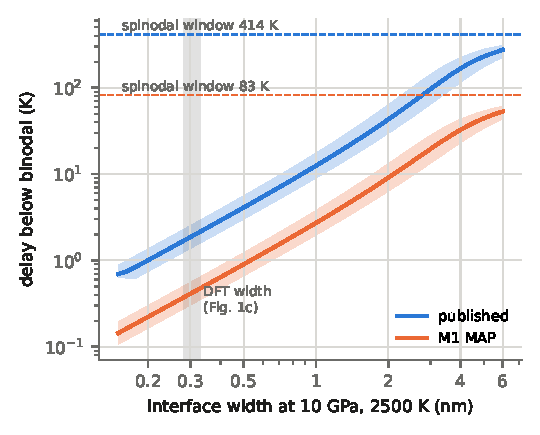
\includegraphics[width=0.6\columnwidth]{fig5_3_nucleation_delay}
\thesiscaption{Nucleation ends the metastable delay close to the binodal.}{Undercooling below
the binodal at which a 3\,wt\% parcel at 2\,GPa nucleates, against the 10--90\% interface width
at 10\,GPa and 2500\,K, for the published fit (blue) and refit M1 at its MAP (orange). Solid
lines are band medians. Bands span $W^*/k_{\rm B}T = 69$--$123$ and molar volume $\pm30\%$.
Dashed lines mark each binodal--spinodal window (\pubIntTwo{}\,K published, \winMOneMap{}\,K
M1). The grey band is the width of the simulated profile.}\label{fig:nucleation}
\end{figure}

\section{Cooling Paths of a Closed Parcel}\label{sec:parcel}

Figure~\ref{fig:parcel} follows a closed 3\,wt\% parcel at 2\,GPa as it loses heat. Sensible
heat comes from the \Atm{} end members, liquid MgSiO$_3$ (\cpSilicate{}\,kJ\,kg$^{-1}$\,K$^{-1}$)
and ideal-gas H$_2$ (\cpHydrogen{}\,kJ\,kg$^{-1}$\,K$^{-1}$ at 3000\,K). They are weighted by
mass, without a pressure correction. Hydrogen then supplies \cpHydrogenShare{}\% of the sensible
heat capacity of a 3\,wt\% parcel. For comparison, \cite{rogers2025} take
1.195\,kJ\,kg$^{-1}$\,K$^{-1}$ for the silicate melt. If the parcel stayed homogeneous to the
spinodal and then separated, it would release \recalPubHeat{}\,MJ\,kg$^{-1}$ at once and reheat
by \recalPubJump{}\,K (refit M1: \recalMOneHeat{}\,MJ\,kg$^{-1}$, \recalMOneJump{}\,K). Limited
by nucleation, the parcel separates \nucPubOnset{}\,K below the binodal, releases
\nucPubHeat{}\,kJ\,kg$^{-1}$ and reheats by only \nucPubJump{}\,K. Its path is then
indistinguishable from equilibrium. All paths reach the same final state after the same heat
loss (\pathFinalPub{}\,MJ\,kg$^{-1}$ to 2700\,K): delay changes when heat is released, not how
much.

\begin{figure}[t]
\centering
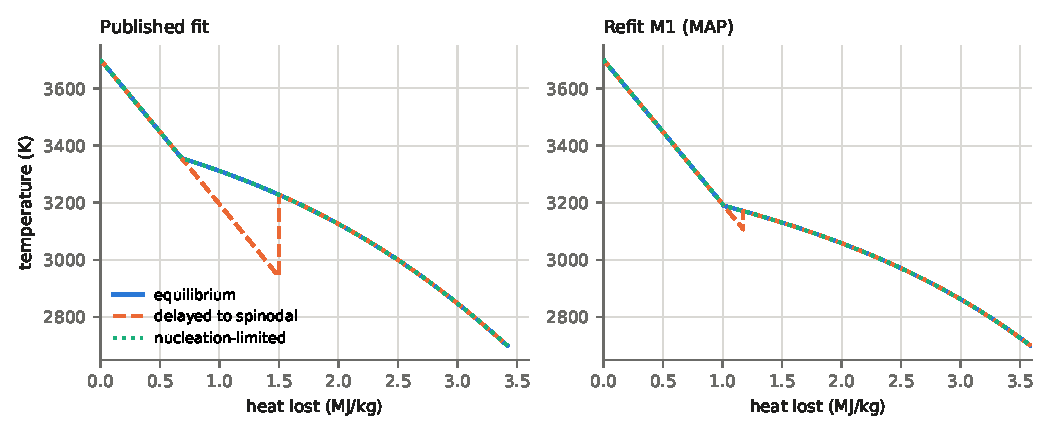
\includegraphics[width=\columnwidth]{fig5_1_parcel_paths}
\thesiscaption{Cooling paths of a closed 3\,wt\% parcel at 2\,GPa.}{Temperature against heat
lost from 3700\,K for the published fit (left) and refit M1 at its MAP (right). Solid lines show
equilibrium separation. Dotted lines show nucleation-limited separation, which overlies the
equilibrium path. Dashed lines show a mean-field bound that nucleation pre-empts: separation
delayed to the spinodal, which would reheat the parcel by \recalPubJump{}\,K (published fit) or
\recalMOneJump{}\,K (refit M1).}\label{fig:parcel}
\end{figure}

\section{A Convecting Interior Releases Exsolution Heat}\label{sec:interior}

In a convecting interior every parcel reaches the top, where the melt meets the envelope. The
envelope already provides the hydrogen-rich phase, so no nucleation is needed there. Deeper
layers are hotter and, because the critical temperature falls with pressure, more miscible.
The interior composition therefore follows the hydrogen-poor binodal at the top, and the
exsolved hydrogen joins the envelope.

Over the first 300\,K of cooling below the binodal, a 3\,wt\% interior with refit M1 at 2\,GPa
loses \intExsolvedThree{}\% (\intExsolvedThreeLo{}--\intExsolvedThreeHi{}\%) of its hydrogen
and releases \intPerKgThree{}\,MJ per kg of it. This heat is \intRatioThree{}
(\intRatioThreeLo{}--\intRatioThreeHi{}) times the sensible heat lost over the same interval by
the interior and the hydrogen it has exsolved, which we let cool with the top of the interior;
for 1\,wt\% it is \intRatioOne{} (\intRatioOneLo{}--\intRatioOneHi{}) times (published fit,
3\,wt\%: \intPubRatioThree{}). Without the exsolved hydrogen in the sensible heat, the ratio at
3\,wt\% is \intInteriorOnlyThree{} (\intInteriorOnlyThreeLo{}--\intInteriorOnlyThreeHi{}). The
ratio also depends on the chosen interval. About half of the exsolution heat of the first
300\,K is released in the first 100\,K, while the sensible heat grows in proportion to the
cooling. The median ratio is therefore \intRatioThreeHundredK{} over the first 100\,K and
\intRatioThreeSixHundredK{} over the first 600\,K; for the published fit it is
\intPubRatioThreeHundredK{} and \intPubRatioThreeSixHundredK{}.

Just below the binodal, exsolution adds up to \intGammaThree{}
(\intGammaThreeLo{}--\intGammaThreeHi{}) times the sensible heat capacity at 3\,wt\%
(Figure~\ref{fig:interior}b). The effective heat capacity of the interior there is thus up to
\intCeffThree{} (\intCeffThreeLo{}--\intCeffThreeHi{}) times the sensible one, and the interior
cools markedly more slowly while it exsolves.

These numbers rest on five assumptions, and each one shifts them. First, overturn is fast
compared with cooling, so the interior stays uniform. Second, the top pressure stays at
2\,GPa. In the evolution of \cite{rogers2025}, the binodal pressure rises from 0.9 to 4.9\,GPa
while its temperature falls by 925\,K. At higher pressure the melt at the top dissolves more
hydrogen. A rise at that rate lowers the exsolution heat over the first 300\,K by
\risePressMOne{}\% for refit M1 (median) and by \risePressPub{}\% for the published fit. Third,
the whole interior cools by as much as its top. On an adiabat the mean temperature falls faster
than the top temperature, and the ratio to sensible heat falls by the same factor. A factor of
1.3, for example, lowers the median ratio from \intRatioThree{} to \intRatioThreeAdiabat{}.
Fourth, the model includes no gravitational energy from rising hydrogen or settling melt; in
\cite{rogers2025} that energy is part of the gravitational term. Fifth, the exsolved hydrogen
ends as pure H$_2$.

Near the binodal the coexisting hydrogen-rich phase still carries much silicate. In refit M1 it
holds only \intUpperWtThree{}\,wt\% hydrogen 1\,K below the binodal (median). Suppose the
hydrogen leaves the melt as that phase. Each kilogram of hydrogen then releases only
\intPhasePerKgThree{}\% of the pure-H$_2$ heat. The departing phase also removes silicate, so
more hydrogen must leave per kelvin of cooling. The heat released per kelvin is then
\intPhasePerKThree{}\% of the pure-H$_2$ value 1\,K below the binodal and
\intPhasePerKHundredThree{}\% at 100\,K below it. Exsolution then adds at most
\intPhaseGammaThree{} (\intPhaseGammaThreeLo{}--\intPhaseGammaThreeHi{}) times the sensible
heat capacity, and the ratio over 300\,K falls to \intPhaseRatioThree{}
(\intPhaseRatioThreeLo{}--\intPhaseRatioThreeHi{}). If the hydrogen instead joins an envelope
that is already at the coexisting composition, it releases \intNetFracThree{}\% of the
pure-H$_2$ heat 1\,K below the binodal, and exsolution adds at most \intNetGammaThree{}
(\intNetGammaThreeLo{}--\intNetGammaThreeHi{}) times the sensible heat capacity. The remainder
appears higher in the envelope as the silicate rains out (Section~\ref{sec:heat_discussion}).
The interior cools more slowly in every case, but the pure-H$_2$ factors are upper bounds for
the interior itself.

At the scale of the whole planet the term is smaller. We digitized the fiducial evolution of
\cite{rogers2025} (6\,$M_\oplus$ with 3\% hydrogen; their Figures~5 and~6). Along it we
integrate our partial molar internal energies, the enthalpies minus the pressure--volume term,
which is the energy basis of their budget. The planet exsolves \planetExsolvedPct{}\% of its
hydrogen between 5\,Myr and 9\,Gyr. Across the class-M1 refits that use the enthalpy data, the
heat is \planetRadiatedLo{}--\planetRadiatedHi{}\% of the energy the planet radiates over that
time and \planetGravityLo{}--\planetGravityHi{}\% of its gravitational energy release, which
supplies most of the luminosity. It is \planetThermal{} (\planetThermalLo{}--\planetThermalHi{})
times the thermal-energy loss in the same budget, and \planetSensible{}
(\planetSensibleLo{}--\planetSensibleHi{}) times the sensible heat the interior loses as it
cools with the binodal. The estimate is a scaling, not a prediction. The thermal history comes
from the 2025 phase diagram. Its binodal path falls below the critical temperature of the 2026
fit only after about \planetCrossPubGyr{}\,Gyr, when \planetCrossPubExsolved{}\% of that
exsolution has already happened. For refit M1 fitted to all data it stays above the critical
temperature throughout, but \planetCrossPooledPct{}\% of the samples of all M1 fits with
enthalpy data fall below it. A consistent planetary estimate needs an evolution model that uses
the same free energy for both. No evolution model we checked includes the heat of exsolution
\cite{rogers2025,rogers2026,young2026,tang2026,tejada2026}.

\begin{figure}[t]
\centering
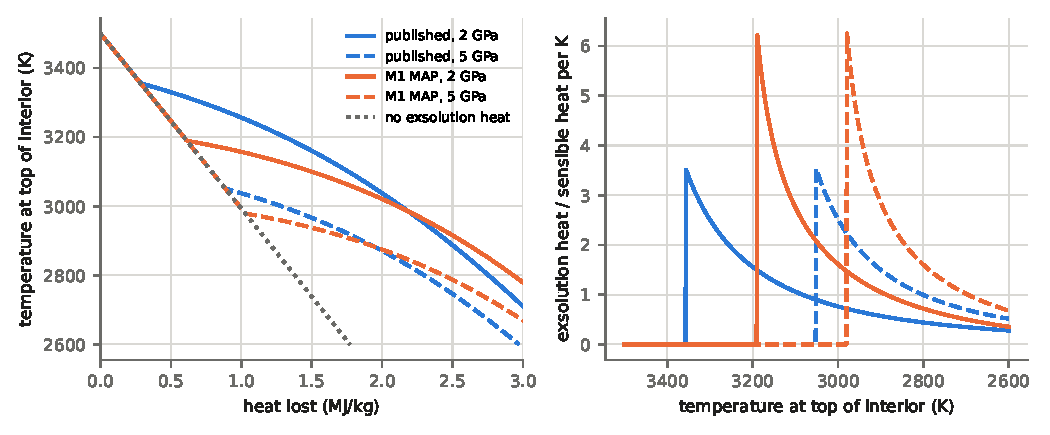
\includegraphics[width=\columnwidth]{fig5_2_interior}
\thesiscaption{Exsolution heat in a convecting 3\,wt\% interior.}{Published fit (blue) and
refit M1 at its MAP (orange), with the top at 2\,GPa (solid) and 5\,GPa (dashed). (a)
Temperature at the top of the interior against heat lost per kg of system. The dotted line is
the sensible heat alone, which is the same for all four cases. (b) Exsolution heat per kelvin
of cooling divided by the sensible heat capacity. The effective heat capacity is one plus this
ratio.}\label{fig:interior}
\end{figure}

The \Atm{} solver reproduces the mixing enthalpy along one published-fit parcel path to
$\replayDiff{}$ over \replayRows{} solves (Appendix~\ref{app:repro}). The interior paths and
the nucleation onsets are not replayed through the solver.
